\documentclass[12pt]{article}
\usepackage[utf8]{inputenc}
\usepackage[spanish]{babel}
\usepackage{amsmath}
\usepackage{amsthm}
\usepackage{hyperref}
\usepackage{graphicx}
\usepackage{color}
\usepackage{float}
\usepackage{multicol}
\usepackage{enumerate}
\usepackage{anyfontsize}
\usepackage{anysize}
\usepackage{tikz}
\usepackage{siunitx}
\usepackage{gensymb}
\usetikzlibrary{arrows.meta, positioning}
\setlength{\parskip}{1em}
\spanishdecimal{.}
\title{\vspace*{-2cm}División política de México\vspace{-5ex}}
\date{\today}
\begin{document}
\maketitle

Identifica mediante el número a cada estado de la República Mexicana y relaciona su capital con el mismo número:
\begin{table}[H]
\centering
\begin{tabular}{p{5cm} p{2cm} p{6cm}}
( ) Aguascalientes & & ( ) Puebla de Zaragoza \\
( ) Baja California & & ( ) Guanajuato \\
( ) Baja California Sur & & ( ) Monterrey \\
( ) Campeche & & ( ) Santiago de Querétaro \\
( ) Chiapas & & ( ) Mérida \\
( ) Chihuahua & & ( ) Villahermosa \\
( ) Ciudad de México &  & ( ) Hermosillo \\
( ) Coahuila & & ( ) Pachuca de Soto \\
( ) Colima & & ( ) Tepic \\
( ) Durango & & ( ) Saltillo \\
( ) Guanajuato & & ( ) Tuxtla Gutiérrez \\
( ) Guerrero & & ( ) Ciudad Victoria \\
( ) Hidalgo & & ( ) Aguascalientes \\
( ) Jalisco & & ( ) Mexicali \\
( ) México & & ( ) Oaxaca de Juárez \\
( ) Michoacán & & ( ) Cuernavaca \\
( ) Morelos & & ( ) Xalapa-Enríquez \\
( ) Nayarit & & ( ) San Francisco de Campeche \\
( ) Nuevo León & & ( ) Chihuahua \\
( ) Oaxaca & & ( ) Colima \\
( ) Puebla & & ( ) Tlaxcala de Xicohténcatl \\
( ) Querétaro & & ( ) Victoria de Durango \\
( ) Quintana Roo & & ( ) Guadalajara \\
( ) San Luis Potosí & & ( ) La Paz \\
( ) Sinaloa & & ( ) Ciudad de México \\
( ) Sonora & & ( ) Zacatecas \\
( ) Tabasco & & ( ) Chilpancingo de los Bravo \\
( ) Tamaulipas & & ( ) Morelia \\
( ) Tlaxcala & & ( ) San Luis Potosí \\
( ) Veracruz & & ( ) Culiacán Rosales \\
( ) Yucatán & & ( ) Toluca de Lerdo \\
( ) Zacatecas & & ( ) Chetumal \\
\end{tabular}
\end{table}


\begin{figure}[H]
    \centering
    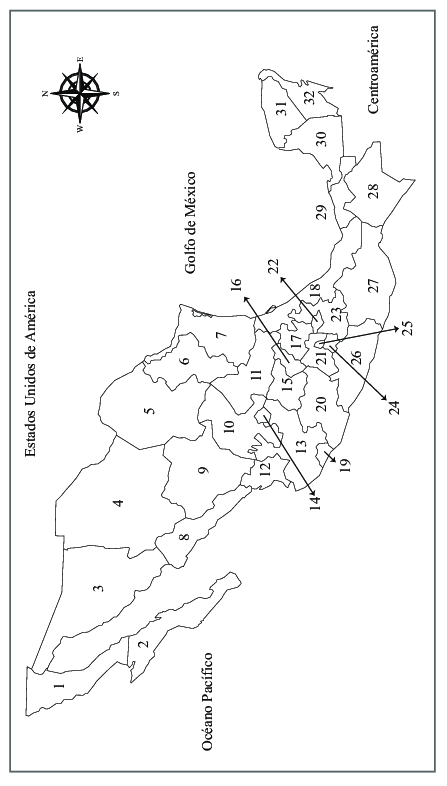
\includegraphics[scale=1]{Mexico_Estados.png}
\end{figure}

\end{document}